\documentclass[../main.tex]{subfiles}

\begin{document}
Let $f(x) = \sqrt{4 - x^2}$. Domain of $f$ is $[-2, 2]$.
\begin{itemize}
    \item $x = -2$ is the left end point of Dom($f$).
    \item $x = 2$ is the right end point of Dom($f$).
    \item Any $x$ with $-2 < x < 2$ is called an interior point of Dom($f$).
\end{itemize}

\begin{definition}
    A function $f$ is \textbf{continuous} at an interior point $c$ of its domain if
    \[
        \lim_{x \to c} f(x) = f(c)
    \]
\end{definition}

Note that $f$ is discontinuous at $c$ if
\begin{itemize}
    \item[i)] either $\lim_{x \to c} f(x)$ does not exist.
    \item[ii)] or $\lim_{x \to c} f(x)$ exists but is not equal to $f(c)$.
\end{itemize}

\begin{figure}[htbp]
    \centering
    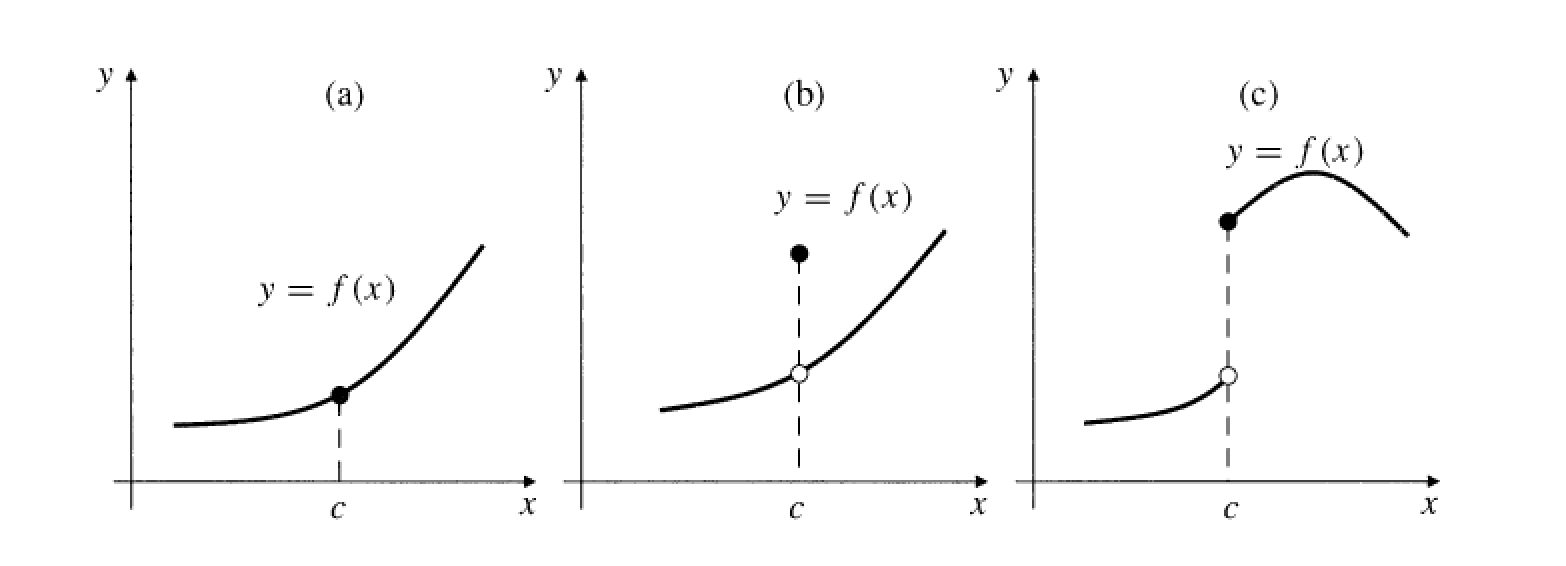
\includegraphics[width=0.95\textwidth]{adams-1-4-fig17}
    \caption{a) $f$ is continuous at $c$, b) $f$ is discontinuous at $c$ because of (ii), c) $f$ is discontinuous at $c$ because of (i)}
\end{figure}

\begin{definition}
    $f$ is \textbf{right continuous} at $c$ if
    \[
         \Lim{x}{c^+} f(x) = f(c)
    \]
    and \textbf{left continuous} at $c$ if
    \[
        \Lim{x}{c^-} f(x) = f(c).
    \]
\end{definition}

If Dom($f$)$= [a, b]$ then
\begin{itemize}
    \item $f$ is continuous at $a$ if it is right continuous at $a$
    \item $f$ is continuous at $b$ if it is left continuous at $b$
\end{itemize}

\begin{example}
    Show that $f(x) = \sqrt{4 - x^2}$ is continuous at every point of its domain.
    \begin{figure}[htbp]
        \centering
        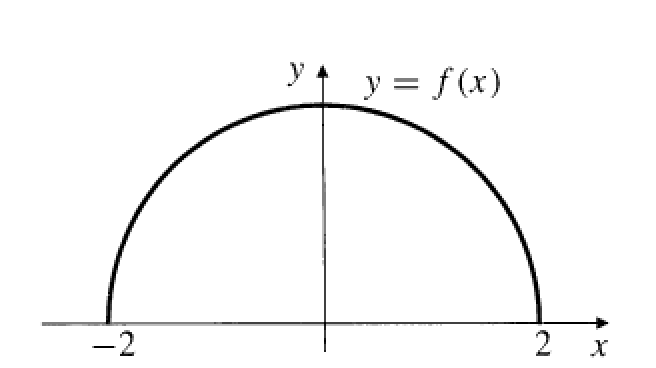
\includegraphics[scale=0.5]{adams-1-4-fig19}
        \caption{$f(x) = \sqrt{4 - x^2}$}
    \end{figure}
\end{example}

\begin{definition}
    $f$ is called a continuous function if $f$ is continuous at every pt of its domain.
\end{definition}

According to this definition $f(x) = \frac{1}{x}$ is continuous!!! $0$ is not in domain of $f$. So we say $f$ is undefined rather than discontinuous at $0$.

\begin{example}
    \begin{figure}[H]
        \centering
        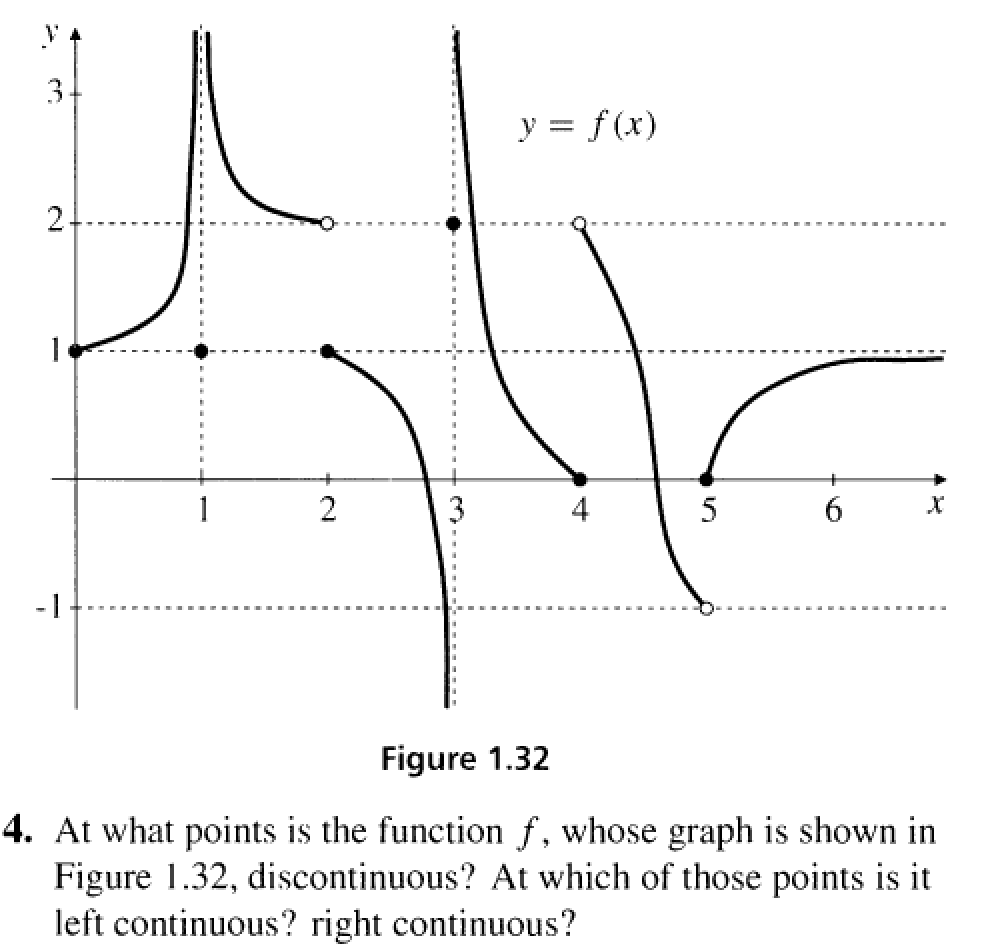
\includegraphics[scale=.5]{adams-1-5-ex4}
    \end{figure}
\end{example}


\textbf{There are lots of continuous functions:}
\begin{itemize}
    \item polynomials,
    \item rational functions,
    \item rational powers $x^{m/n}$
    \item trig functions
    \item absolute value function $\abs{x}$
\end{itemize}

\textbf{Combining continuous functions:}
If $f$ and $g$ are continuous at $c$ then
\begin{itemize}
    \item $f + g$, $f - g$, $f g$, are continuous at $c$,
    \item if $k$ is constant then $k f$ is continuous at $c$,
    \item $\frac{f}{g}$ continuous at $c$ provided that $g(c) \neq 0$.
    \item $f(x)^{1/n}$ continuous at c provided that $f(c)>0$ if $n$ is even.
\end{itemize}

\textbf{Composites of continuous funcs are continuous}

If $g$ is continuous at $c$ and $f$ is continuous at $g(c)$ then $f \circ g$ is continuous at $c$.

\begin{example}
    Find $m$ so that
    \[
        g(x) = \begin{cases}
            x-m, &\text{ if }x < 3,\\
            1-mx, &\text{ if }x \geq 3\\
        \end{cases}
    \]
    is continuous for all $x$.
\end{example}

\textbf{Continuous extensions and removable discontinuities}

If $f$ is not defined at $c$ but $\lim_{x \to c} f(x) = L$ is defined then we can define a new function
\[
    F(x) =
    \begin{cases}
        f(x), &\text{ if } x \neq c\\
        L, &\text{ if } x =c\\
    \end{cases}
\]
$F$ is continuous at $c$ and is called \textbf{continuous extension} of $f$ to $x=c$.
\begin{example}
    The function $f(x) = \dfrac{x^2 - x}{x^2 - 1}$ is not defined at $x=1$ but has a continuous extension $F(x) = \dfrac{x}{x+1}$ to $x=1$.
\end{example}

If a function is undefined or discontinuous at $c$ but can be redefined at $c$ then we say $f$ has a \textbf{removable discontinuity} at $c$.

\begin{example}
    The function $f(x) = \dfrac{1}{x^2}$ is not defined at 0 but there is no way of redefining $f$ at 0 so that $f$ becomes continuous at 0.
\end{example}

\textbf{Continuous Functions on Closed Intervals [a, b] are bounded.}
\begin{theorem}
    If $f$ is continuous on the closed interval $[a, b]$ then there exist numbers $p$ and $q$ s.t.
    \[
        f(p) \leq f(x) \leq f(q)
    \]
    for all $x$ in $[a, b]$.
    $f(p)$ is the \textbf{aboslute minimum value} and $f(q)$ is the \textbf{absolute maximum value}.
\end{theorem}
How to find $p$ and $q$? This is just an existence theorem.

\begin{example}
    The conclusions of the theorem may fail if the function $f$ is not continuous or the interval is not closed. Do Figure 1.25 and Figure 1.27.
    \begin{figure}[H]
        \centering
        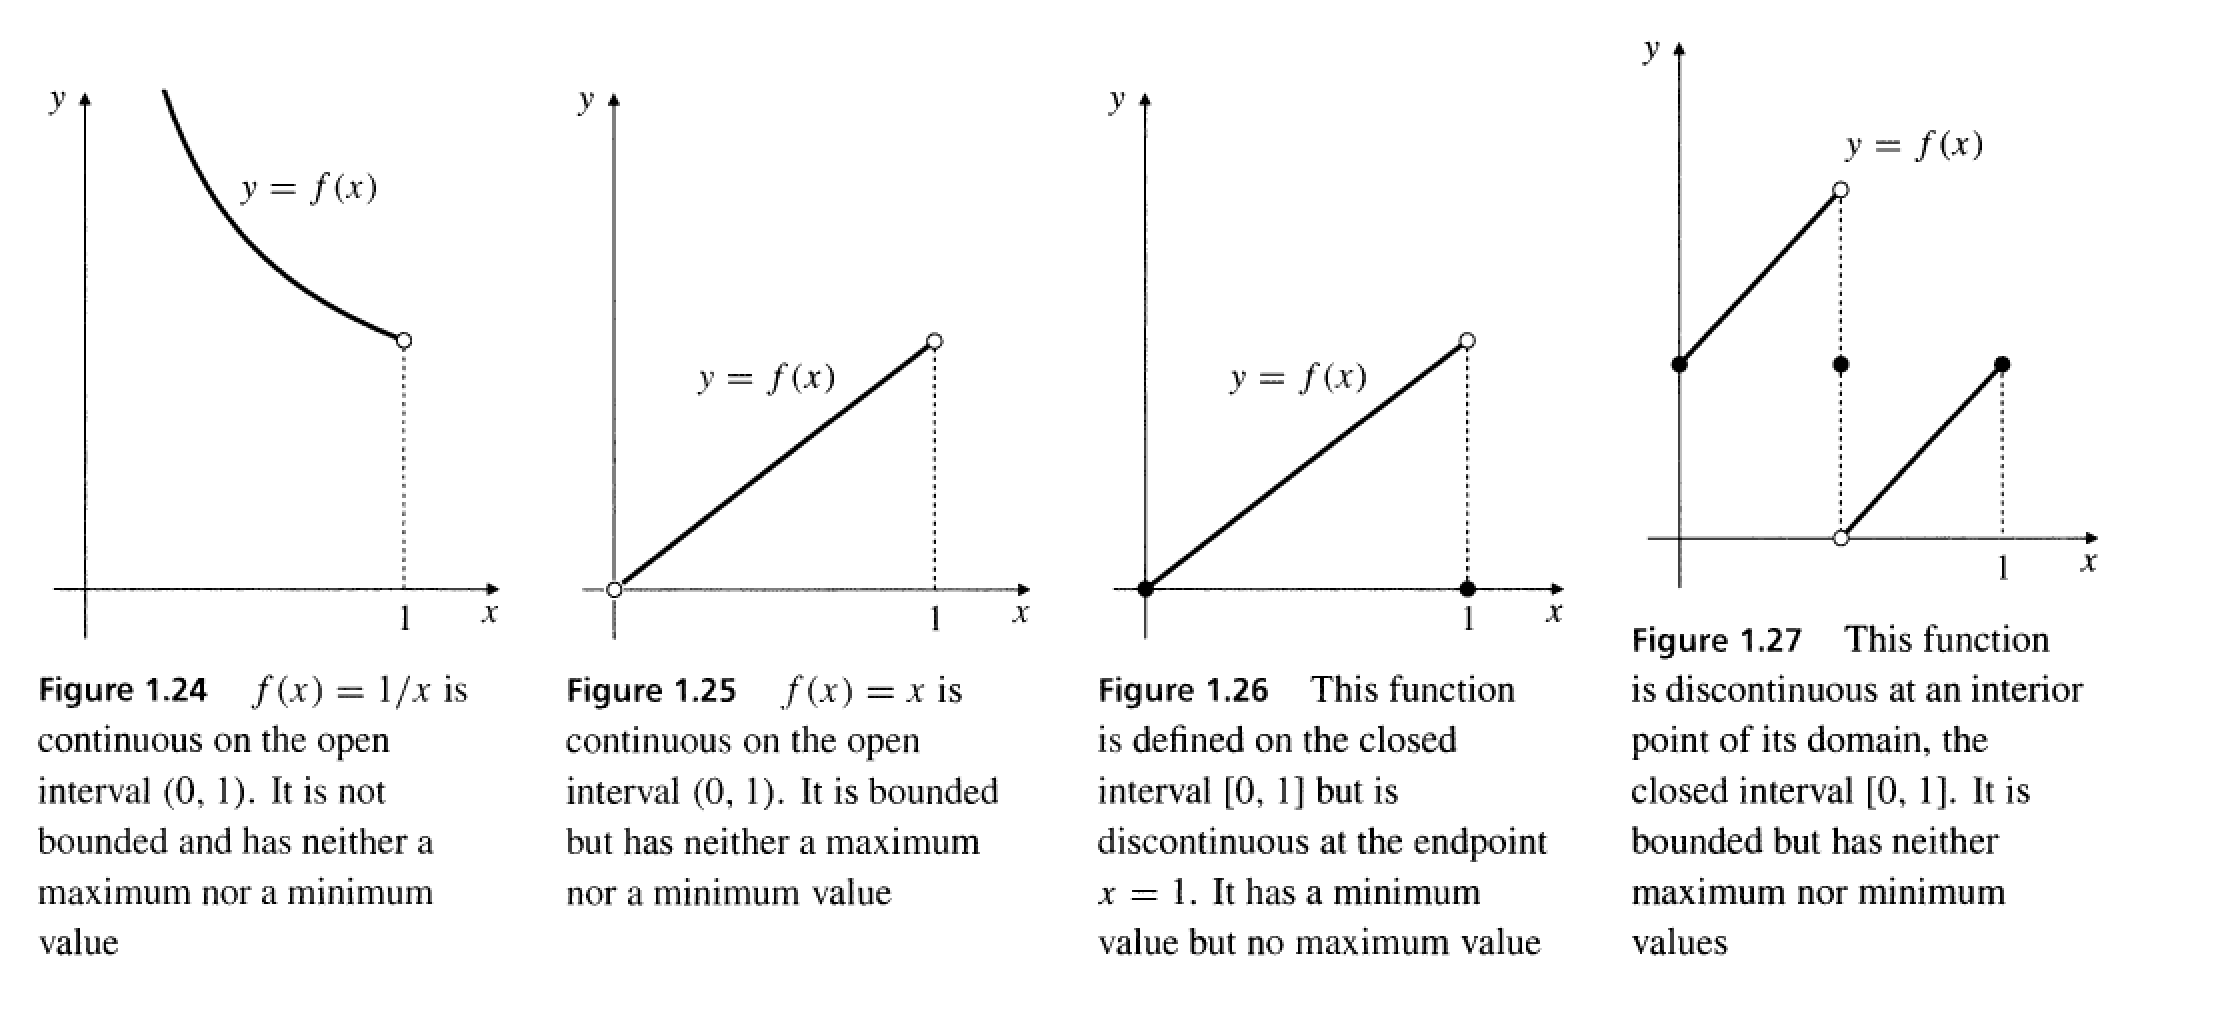
\includegraphics[scale=.35]{adams-1-4-fig24}
    \end{figure}
\end{example}

\begin{theorem}[Intermediate Value Theorem]
    If $f$ is continuous on $[a, b]$ and if $s$ is between $f(a)$ and $f(b)$ then there exists $c$ in $[a, b]$ s.t. $f(c) = s$.
\end{theorem}

\begin{figure}[H]
    \centering
    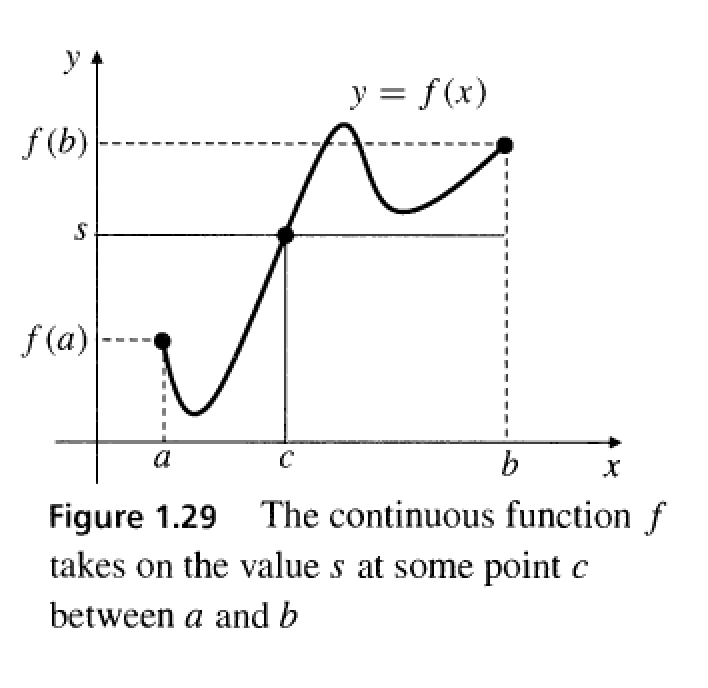
\includegraphics[scale=.5]{adams-1-4-fig29}
\end{figure}

\begin{example}
    Show that the equation $x^3 - x - 1 = 0$ has a solution in the interval $[1, 2]$.
\end{example}

\begin{solution}
    $f(x) = x^3 - x - 1$ is a polynomial and hence continuous. $f(1) = -1$ and $f(2) = 5$. Since $0$ lies between $-1$ and $5$, the intermediate value theorem assures us that there must be a number $c$ in $[1, 2]$ such that $f(c) = 0$.
\end{solution}
\end{document}